\section{The mathematical model for Alzheimer Disease}
As mentioned above, in our brain there exists a protein called beta amyloid peptide ($\mathrm{A} \beta$). Also healthy brains produce this protein in monomeric form, when the mechanism breaks down \(\beta\) starts to auto agglomerate and to form senile plaques. The toxic polymers are the intermediate oligomeric formulation which produces the death of neurons. This is because when these polymers develop they produce a toxic mechanism inside the brain that produces the death of neurons. However the causes of the AD are not yet completely known, researchers try to study this phenomena but the problem is that these intermediate polymers decay very soon in other longer ones. From experiments it's not easy to study  the process of coagulation, therefore the mathematical model helps us to study this process. An assumption that we will make is that 'large' assemblies do not aggregate with each other.
\subsection{Model for the brain}
The portion of cerebral tissue considered  in the following is represented by a bounded smooth region $\Omega_{0}\subset \mathbb{R}^3$, whereas the neurons are represented by a family of regular region $\Omega_{j}$ such that \\
(i) $\bar\Omega_{j}\subset \Omega_{0}$  if   $j=1,2,\dots,\bar{M}$\\
(ii) $\bar\Omega_{i}\cap \bar\Omega_{j}= \emptyset$  if $i\neq j$\\
Let us set 
$$
\Omega := \Omega_{0}
\bigcup_{j=1}^{\bar M} \bar\Omega_{j}
$$
\begin{figure}[H]
    \scalebox{.3}{\incfig{drawing}}
    \label{fig:riemmans-theorem}
  \end{figure}
and consider the vector-valued function $u=(u_1,\dots, u_M)$, where $u_j=u_j(t,x)$ $(t\geq 0, t\in \mathbb{R}$ and $x\in \Omega)$ is the molar concentration at the point $x$ and at the time $t$ of an \(\beta\) assembly of $j$ monomers, while $u_M$ takes into account the aggregation of more than $M-1$ monomers. With the definition of $u_M$ we are assuming that 'large' assemblies do not aggregate to each other.\\
In this section we briefly present the modelization of our problem. We are considering three different stages of the aggregation of our \(\beta\): we can model its concentration with $u_{i}$ with $1\leq i \leq m < M$.
The $u_{1}$ describes the concentration of monomers with the following Diffusion-Reaction equation: 
$$
\frac{\partial u_{1}}{\partial t}(t, x)-d_{1} \Delta_{x} u_{1}(t, x)+u_{1}(t, x) \sum_{j=1}^{M} a_{1, j} u_{j}(t, x)=0\\
$$
We don't have the gain term on the righten side because there does not exist two monomers that coagulate to form a single one.
To solve this equation we have to impose boundary conditions and initial conditions.
On the external boundary we assume homogeneous Neumann condition, it is meant to artificially isolate the portion of tissue considered from its environment:
$$
\frac{\partial u_1}{\partial v} \equiv \nabla_{x} u_1\cdot n=0 \quad \text { on }[0, T] \times \partial \Omega$$
We are practically imposing that the flux on external fixed boundary is equal to zero: we are isolating our portion of cerebral tissue from the rest of the world.
We have to put the boundary conditions also on the boundaries of the neurons $\partial\Omega_{j}$:
$$ 
\frac{\partial u_{1}}{\partial v} \equiv \nabla_{x} u_1 \cdot n= \psi_{j} \quad \text { on } \partial\Omega_{j}
$$
This physically models the fact that the neurons produce \(\beta\) in monomeric form. The function $\psi$ is a smooth function and it represents the quantity of \(\beta\) which is produced by the membrane of the neuron, it is a given of the problem.\\
We now model a portion of the cerebral tissue with a bounded open set $\Omega$ in $\mathbb{R}^{3}$ with a smooth boundary $\partial \Omega$. The neurons in our model will be represented as holes in this domain which are distributed periodically and which have characteristic dimension $0<\epsilon<1$. The set of the domain with the holes is called the perforated domain.
We assume that the membrane of the neurons (holes) produces $\mathrm{A} \beta$ and that at time $t=0$ there is no production of  $\mathrm{A} \beta$ from the holes. \\
Let $Y$ be the unit periodicity cell $\left[0,1\left[{ }^{3}\right.\right.$ having the paving property. 
Let us denote by $T$ an open subset of $Y$ with a smooth boundary $\Gamma$, such that $\bar{T} \subset \operatorname{Int} Y$, this means that $T$ can not intersect the boundary of our set $Y$. We call with $Y^{*}=Y \backslash T$ the material part, the "solid part" of our brain.
\begin{figure}[H]
   \centering
   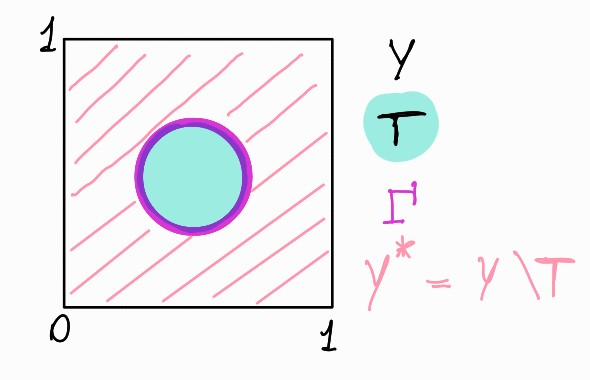
\includegraphics[width=7cm]{unitcellMS.jpg}
   \caption{Unit cell $Y$}
    \label{fig:Y}
\end{figure}

Starting from this we create a perforated domain: we perforate $\Omega$ by removing from it a set $T_{\epsilon}$ of periodically distributed holes defined as before. The set $T$ represents a generic neuron, and $Y^{*}$ the supporting cerebral tissue. We define $\tau(\epsilon \bar{T})$ to be the set of all translated images $\epsilon \bar{T}$ of the form $\epsilon(k+\bar{T}), k \in \mathbb{Z}^{3}$. Then,

\[ T_{\epsilon}:=\Omega \cap \tau(\epsilon \bar{T}) . \] is the set of all the holes in our domain.

Introduce now the periodically perforated domain $\Omega_{\epsilon}$ defined by

$$
\Omega_{\epsilon}=\Omega \backslash \bar{T}_{\epsilon} .
$$
which represent all the set outside the holes.\\

\begin{figure}[H]
   \centering
   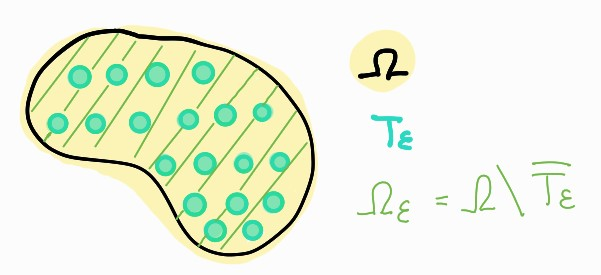
\includegraphics[width=7cm]{periodicallyperforateddomain.jpg}
   \caption{Periodically perforated domain $\Omega$}
    \label{fig:Omega_epsilon}
\end{figure}

We ensure that there exists a "security zone", this is necessary to extend all the functions which live in the solid part also in the holes.
\begin{equation}
  \exists \delta>0 \text { such that dist }\left(\partial \Omega, T_{\epsilon}\right) \geq \delta
\label{eq 8}\end{equation}
Therefore we can assume that $\Omega_{\epsilon}$ is connected. In this scenario there are two boundaries, an internal one $\Gamma_{\epsilon}$, defined by:
$$
\Gamma_{\epsilon}:=\cup\{\partial(\epsilon(k+\bar{T})) \mid \epsilon(k+\bar{T}) \subset \Omega\}
$$
and an external one that is the fixed exterior boundary denoted by $\partial \Omega$:
$$
\partial\Omega_{\epsilon}=\partial\Omega+\Gamma_{\epsilon}
$$
\begin{figure}[H]
   \centering
   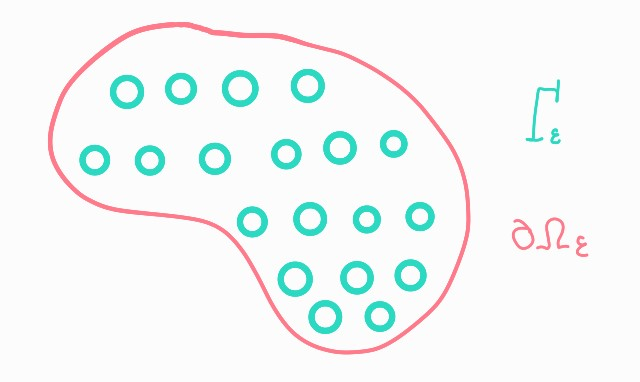
\includegraphics[width=7cm]{boundary.jpg}
   \caption{Periodically perforated domain $\Omega$}
    \label{fig:Omega_epsilon2}
\end{figure}
It is also known that:
\begin{equation}
  \lim _{\epsilon \rightarrow 0} \epsilon\left|\Gamma_{\epsilon}\right|_{N-1}=|\Gamma|_{N-1} \frac{|\Omega|_{N}}{|Y|_{N}}
\label{eq 9}\end{equation}
where $|\cdot|_{N}$ is the $N$-dimensional Hausdorff measure.\\ Our aim is to pass from the microscopic scale to the macroscopic, that is, we are looking at our brain from 'very high' and we obtain it by performing $\epsilon \rightarrow 0$ which is the scale where clinical data exists. This process is called homogenization theory and it is a mathematical technique that gives us some mathematical tools to perform this sort of average.
\subsection{The equations}
The system that describes the evolution of monomers is the following:
\begin{equation}
    \begin{cases}
    \frac{\partial u_{1}^{\epsilon}}{\partial t}(t, x)-d_{1} \Delta_{x} u_{1}^{\epsilon}(t, x)+u_{1}^{\epsilon}(t, x) \sum_{j=1}^{M} a_{1, j} u_{j}^{\epsilon}(t, x)=0 & \text { in }[0, T] \times \Omega_{\epsilon}\\
    \frac{\partial u^{\epsilon}_1}{\partial v} \equiv \nabla_{x} u^{\epsilon}_1\cdot n=0 & \text { on }[0, T] \times \partial \Omega\\
    \frac{\partial u^{\epsilon}_{1}}{\partial v} \equiv \nabla_{x} u^{\epsilon}_1 \cdot n=\epsilon \psi\left(t, x, \frac{x}{\epsilon}\right) & \text { on }[0, T] \times \Gamma_{\epsilon}\\
    u_{1}^{\epsilon}(0, x)=U_{1} & \text{ in }\Omega_{\epsilon}
    \end{cases}
\label{eq 10.1}\end{equation}
Note that the $\epsilon$ is put in front of $\psi$ to prevent the divergence of the integral in a further passage, in order to avoid singularities. 
The variable $x$ is called the slow variable and the dependence between $\psi$ and $x$ models the becoming sick . 
$\frac{x}{\epsilon}$ is called the fast scale variable, which represents the microscopic scale because the main variation of our function are on the scale of the neurons, it's in this small scale that we have a very big change.\\
From our assumptions we suppose that for $t>0$ the brain becomes sick. For technically reasons we have to assume some regularity on $\psi$ and $U_1$:
\begin{enumerate}
    \item $\psi\left(t, x, \frac{x}{\epsilon}\right) \in C^{1}(0, T ; B)$ with $B=C^{1}\left[\bar{\Omega} ; C_{\text {\# }}^{1}(Y)\right]$, where $C_{\#}^{1}(Y)$ is the subset of $C^{1}\left(\mathbb{R}^{N}\right)$ of $Y$-periodic functions;
    \item $\psi\left(t=0, x, \frac{x}{\epsilon}\right)=0$
    \item 
$U_{1}$ is a positive constant such that
\begin{equation}
  U_{1} \leq\|\psi\|_{L^{\infty}(0, T ; B)} .
\label{eq 11}\end{equation}
\end{enumerate}
Behind these properties $\psi $ is a generic given function that should be specified in some way if one wants to make the model applicable. We will give an explicit example of it in the last part of the paper.\\
Now we will describe the evolution of oligomers: $1<m<M$. The unknown here is the concentration of a oligomer of generic length $m$
\begin{equation}
    \begin{cases}
        \frac{\partial u_{m}^{\epsilon}}{\partial t}(t, x)-d_{m} \Delta_{x} u_{m}^{\epsilon}(t, x)+u_{m}^{\epsilon}(t, x) \sum_{j=1}^{M} a_{m, j} u_{j}^{\epsilon}(t, x)= \frac{1}{2} \sum_{j=1}^{m-1} a_{j, m-j} u_{j}^{\epsilon} u_{m-j}^{\epsilon} & \text { in }[0, T] \times \Omega_{\epsilon} \\
        \frac{\partial u_{m}^{\epsilon}}{\partial v} \equiv \nabla_{x} u_{m}^{\epsilon} \cdot n=0  & \text { on }[0, T] \times \partial \Omega \\
        \frac{\partial u_{m}^{\epsilon}}{\partial v} \equiv \nabla_{x} u_{m}^{\epsilon} \cdot n=0 & \text { on }[0, T] \times \Gamma_{\epsilon}\\ 
     u_{m}^{\epsilon}(0, x)=0 & \text{ in } \Omega_{\epsilon}
    \end{cases}
\label{eq 12}\end{equation}
In this case we assume homogeneous boundary conditions also on $\Gamma_{\epsilon}$ because we assume that the neurons can't produce \(\beta\) in oligomeric form.
For what it concerns $u_{M}$, it describes the sum of all the densities of all large assemblies of \(\beta\). We are able to do that because in reality when we have a large polymer of \(\beta\) it doesn't  coagulate anymore. 
\begin{equation}
    \begin{cases}
        \frac{\partial u_{M}^{\epsilon}}{\partial t}(t, x)-d_{M} \Delta_{x} u_{M}^{\epsilon}(t, x)= \frac{1}{2} \sum_{\substack{j+k\geq M\\k<M\\j<M}} a_{j, k} u_{j}^{\epsilon} u_{k}^{\epsilon} & \text { in }[0, T] \times \Omega_{\epsilon}\\
        \frac{\partial u_{M}^{\epsilon}}{\partial v} \equiv \nabla_{x} u_{M}^{\epsilon} \cdot n=0  & \text { on }[0, T] \times \partial \Omega
        \\
        \frac{\partial u_{M}^{\epsilon}}{\partial v} \equiv \nabla_{x} u_{M}^{\epsilon} \cdot n=0 & \text { on }[0, T] \times \Gamma_{\epsilon}\\ 
        u_{M}^{\epsilon}(0, x)=0 & \text{ in } \Omega_{\epsilon}
    \end{cases}
    \label{eq 13}
\end{equation}
In this last system there isn't the loss term because they don't coagulate each other.
At this point we want to go from macroscopic to microscopic, trying to compute a sort of average process. Indeed our aim is to perform the homogenization on the set \eqref{eq 10}-\eqref{eq 13} of equations as $\epsilon \rightarrow 0$, however there is not a clear notion of convergence for the sequence $u_j^{\epsilon}$ $1\geq j \geq M$ which is defined on a varying set $\Omega_{\epsilon}$, which also is random perforated.

\begin{theorem} 
    If $\epsilon>0$, the system (10)-(13) has a unique solution
    $$
    \left(u_{1}^{\epsilon}, \ldots, u_{M}^{\epsilon}\right) \in C^{1+\alpha / 2,2+\alpha}\left([0, T] \times \Omega_{\epsilon}\right) \quad(\alpha \in(0,1))
    $$
    such that
    $$
    u_{j}^{\epsilon}(t, x)>0 \text { for }(t, x) \in(0, T) \times \Omega_{\epsilon}, j=1, \ldots, M .
    $$
    \label{thm 4.1}
\end{theorem}
